%#########################################################################
\chapter{Electrostática}
\label{cha:electrostatic}

La electrostática estudia la interacción entre cuerpos cargados 
eléctricamente sin tener en cuenta su movimiento. Esta simplificación 
permite ignorar términos dinámicos asociados a corrientes eléctricas y 
campos magnéticos inducidos.

\

En este capítulo se realizan algunas demostraciones computacionales que 
van desde el cálculo de trayectorias de partículas en campos eléctricos y 
magnéticos, la representación de las líneas de campo y superficies 
equipotenciales de distribuciones de carga, hasta el cálculo de 
capacitancia de algunos sistemas.
%#########################################################################



\
%*************************************************************************
\section{Demostración 1: Espectrómetro de Masas}
\label{sec:DEMO2_01}
\rule{14cm}{0.5mm}

En esta primera demostración será estudiado el espectrómetro de masas. El 
objetivo de este dispositivo es caracterizar partículas cargadas de acuerdo
a su relación carga masa $(q/m)$. Su funcionamiento consiste en la inmersión 
de las partículas en un campo magnético o eléctrico (este caso) y a partir de
las trayectorias obtenidas determinar su relación carga masa (ver figura 
\ref{fig:mass_spectrometer}).

\

Tomando una partícula de masa $m$ y carga $q$ embebida en un campo eléctrico
homogéneo y uniforme $\bds E$, la ecuación de movimiento es


%.........................................................................
%Movement equation
\eq{eq:charged_particle}
{m\dtot{^2\bds r}{t^2} = q\bds E}
%.........................................................................


Tomando el sistema coordenado de tal forma que el campo $\bds E$ esté en la
dirección positiva de y, se obtiene


%.........................................................................
%Mass Spectrometer
\begin{figure}[htbp]
	\centering
	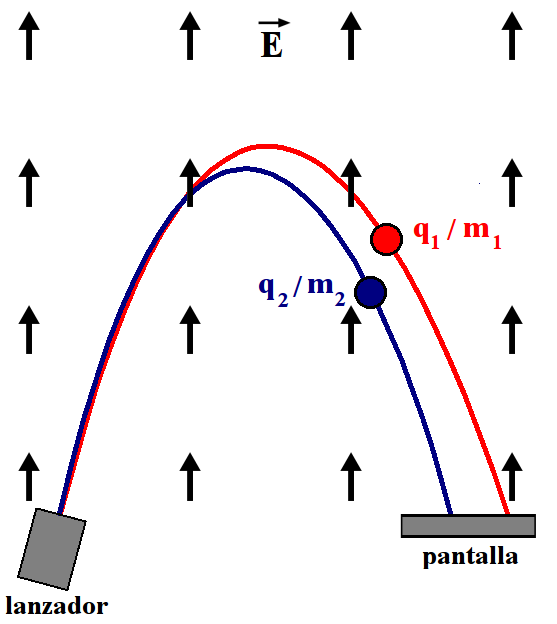
\includegraphics[width=0.50\textwidth]
	{./pictures/mass_spectrometer.png}

	\caption{\small{Espectrómetro de masas.}}
	
	\label{fig:mass_spectrometer}
\end{figure}
%.........................................................................


%.........................................................................
%Movement equations solution
\begin{eqnarray}
\label{eq:x_equation}
x(t) &=& x_0 + v_{x0}t \\
\label{eq:y_equation}
y(t) &=& y_0 + v_{y0}t + \frac{1}{2}\pr{\frac{q}{m}}t^2
\end{eqnarray}
%.........................................................................
donde se ha introducido la posición inicial de la partícula $\bds r(t=0) = 
(x_0, y_0)$ y la velocidad inicial $\bds v(t=0) = (v_{x0}, v_{y0})$.

\

Eliminando el tiempo de las dos ecuaciones se obtiene la siguiente 
trayectoria


%.........................................................................
%Trayectory
\eq{eq:trayectory}
{y(x) = y_0 + \frac{v_{y0}}{v_{x0}}(x - x_0) + 
\frac{1}{2}\pr{\frac{q}{m}} \pr{ \frac{x - x_0}{v_{x0}} }^2}
%.........................................................................

\

En el siguiente código de \python se grafica la trayectoria de dos 
partículas con diferente relación carga masa. La primera tiene una 
relación $q_1/m_1 = -1\mbox{ C}/1 \mbox{ kg}$ y la segunda $q_2/m_2 = 
-1\mbox{ C}/2 \mbox{ kg}$. Ambas partículas se disparan del origen y con 
una elocidad inicial de $\bds v_0 = (1, 2) \mbox{ m/s}$. El campo eléctrico 
tiene una intensidad de $|\bds E| = 1 \mbox{ N/C}$.

\newpage
%ccccccccccccccccccccccccccccccccccccccccccccccccccccccccccccccccccccccccc
%DEMO 2_01
\begin{listing}[style=python]
#!/usr/bin/env python
#==========================================================
# DEMOSTRACION 1
# Espectrometro de masas
#==========================================================
from __future__ import division
import numpy as np
import matplotlib.pylab as plt

#Trayectoria
def trayectory(x):
    y = y0 + vy0/vx0*(x - x0) + 0.5*(q/m)*( (x-x0)/vx0 )**2
    return y
    
#PARTICULA 1
#Carga
q = -1
#Masa
m = 1
#Posicion inicial
x0 = 0
y0 = 0
#Velocidad inicial
vx0 = 1
vy0 = 2
#Valores de X a graficar
X = np.arange( 0, 10, 0.01 )
#Trayectoria
Y = trayectory( X )
#Grafica de trayectoria
plt.plot( X, Y, label='particula 1' )

#PARTICULA 2
#Carga
q = -1
#Masa
m = 2
#Posicion inicial
x0 = 0
y0 = 0
#Velocidad inicial
vx0 = 1
vy0 = 2
#Valores de X a graficar
X = np.arange( 0, 10, 0.01 )
#Trayectoria
Y = trayectory( X )
#Grafica de trayectoria
plt.plot( X, Y, label='particula 2' )

#Limites del eje X
plt.xlim( (0,10) )
#Limites del eje Y
plt.ylim( (0,10) )
plt.legend()
plt.show()
\end{listing}
%ccccccccccccccccccccccccccccccccccccccccccccccccccccccccccccccccccccccccc


El resultado que se obtiene es


%.........................................................................
%Trayectories
\begin{figure}[htbp]
	\centering
	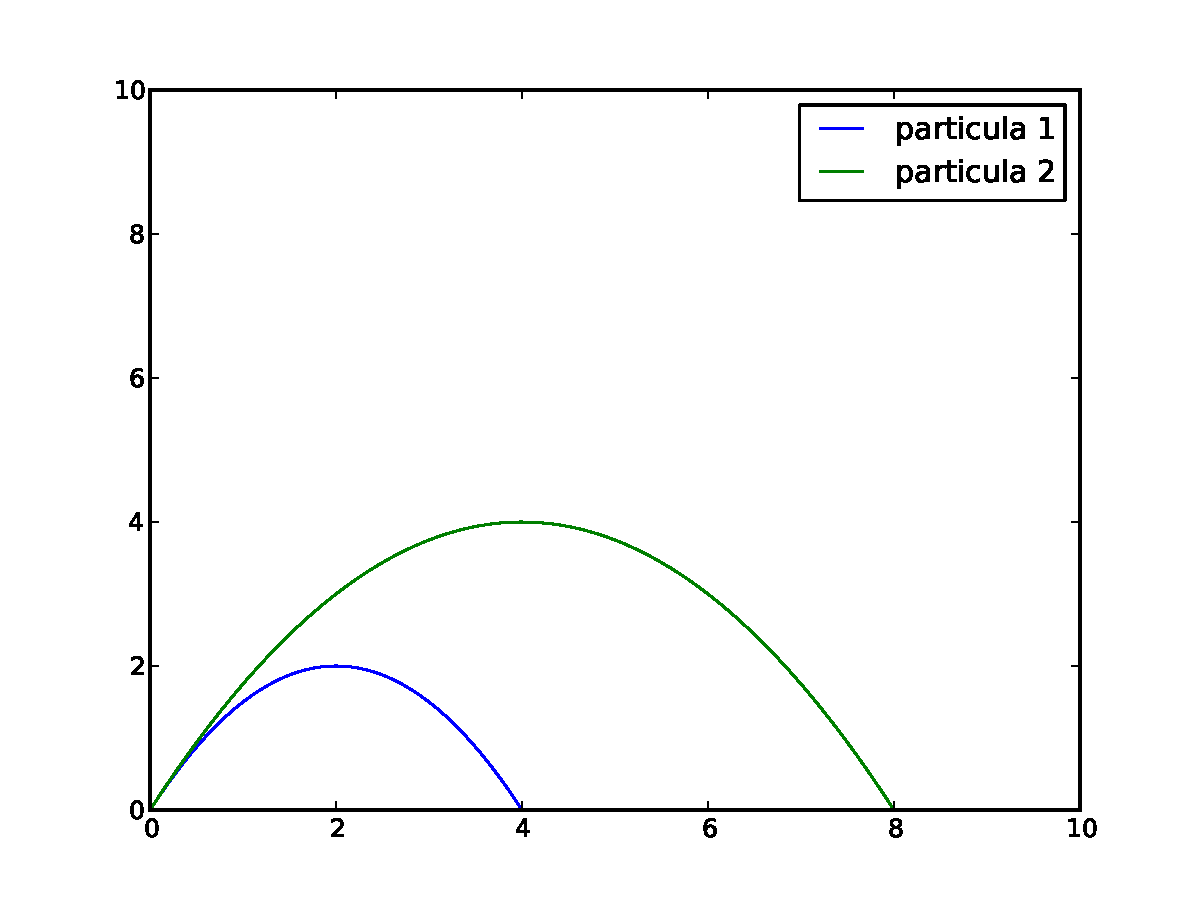
\includegraphics[width=0.8\textwidth]
	{./pictures/demo2_01.pdf}

	\caption{\small{Trayectorias según la relación carga masa de las 
	partículas.}}
	
	\label{fig:trayectories}
\end{figure}
%.........................................................................


La representación de la trayectoria de forma gráfica permite entonces 
comparar directamente con datos medidos en un laboratorio, por ejemplo 
trayectorias de partículas en cámaras de burbujas.

\newpage

A continuación se explica cada componente del código anterior


%ccccccccccccccccccccccccccccccccccccccccccccccccccccccccccccccccccccccccc
%DEMO 2_01
\begin{listing}[style=python, numbers = none]
from __future__ import division
import numpy as np
import matplotlib.pylab as plt
\end{listing}
%ccccccccccccccccccccccccccccccccccccccccccccccccccccccccccccccccccccccccc
En la primera línea se carga el módulo \texttt{division}, este permite a 
\python calcular fracciones de números enteros como cantidades reales. En
la siguiente línea se carga la librería \numpy con el alias de \texttt{np}
y finalmente se carga la librería \matplotlib con el alias de \texttt{plt}.


%ccccccccccccccccccccccccccccccccccccccccccccccccccccccccccccccccccccccccc
%DEMO 2_01
\begin{listing}[style=python, numbers = none]
#Trayectoria
def trayectory(x):
    y = y0 + vy0/vx0*(x - x0) + 0.5*(q/m)*( (x-x0)/vx0 )**2
    return y
\end{listing}
%ccccccccccccccccccccccccccccccccccccccccccccccccccccccccccccccccccccccccc
En esta parte se define la trayectoria de la partícula en el campo 
eléctrico descrito.

%ccccccccccccccccccccccccccccccccccccccccccccccccccccccccccccccccccccccccc
%DEMO 2_01
\begin{listing}[style=python, numbers = none]    
#PARTICULA 1
#Carga
q = -1
#Masa
m = 1
#Posicion inicial
x0 = 0
y0 = 0
#Velocidad inicial
vx0 = 1
vy0 = 2
#Valores de X a graficar
X = np.arange( 0, 10, 0.01 )
#Trayectoria
Y = trayectory( X )
#Grafica de trayectoria
plt.plot( X, Y, label='particula 1' )
\end{listing}
%ccccccccccccccccccccccccccccccccccccccccccccccccccccccccccccccccccccccccc
Se definen las propiedades físicas y cinemáticas de la partícula 1. Su 
carga, su masa, su posición y velocidad inicial. Luego, usando el comando
\texttt{arange} de la librería \numpy, se construye un arreglo de valores 
en el eje X que serán usados para el cálculo de la trayectoria. En este 
caso se toma desde 0 a $10$ m con un salto de $0.01$ m. Finalmente se 
llama la función de la trayectoria de la partícula en todos los valores de
\texttt{X} y se grafica, usando como etiqueta \texttt{label='particula 1'}.


%ccccccccccccccccccccccccccccccccccccccccccccccccccccccccccccccccccccccccc
%DEMO 2_01
\begin{listing}[style=python, numbers = none]
#Limites del eje X
plt.xlim( (0,10) )
#Limites del eje Y
plt.ylim( (0,10) )
plt.legend()
plt.show()
\end{listing}
%ccccccccccccccccccccccccccccccccccccccccccccccccccccccccccccccccccccccccc
Finalmente se usan las funciones de \matplotlib \texttt{xlim} y \texttt{ylim}
para fijar los límites de la ventana de graficación. La función 
\texttt{legend} muestra las etiquetas de las dos trayectorias y finalmente
\texttt{show} muestra en pantalla el resultado.


\rule{14cm}{0.5mm}
%*************************************************************************



\
%*************************************************************************
\section{Demostración 2: Líneas de Campo y Equipotenciales}
\label{sec:DEMO2_02}
\rule{14cm}{0.5mm}


Un campo es una distribución espacial de alguna cantidad física, tal como 
el campo eléctrico y magnético. Este puede ser generado por una fuente, tal
como es el caso del campo electrostático generado por una distribución de 
cargas, o pueden no tener una fuente asociada, como el caso de ondas 
electromagnéticas que viajan libre en el espacio.


En esta demostración se calculará las líneas de campo eléctrico y las 
líneas de equipotencial para una distribución de dos partículas puntuales.
Debido al principio de superposición se tiene entonces


%.........................................................................
%Fields of point particles distribution
\begin{eqnarray}
\label{eq:total_phi}
\varphi_{tot}(\bds r) &=& \varphi_1(\bds r) + \varphi_2(\bds r) \\
\nonumber
&=& \frac{1}{4\pi \epsilon_0}\frac{q_1}{|\bds r - \bds r_1|} + 
\frac{1}{4\pi \epsilon_0}\frac{q_2}{|\bds r - \bds r_2|} \\
\label{eq:total_E}
\bds E_{tot}(\bds r) &=& \bds E_1(\bds r) + \bds E_2(\bds r) \\
\nonumber
&=& \frac{1}{4\pi \epsilon_0}\frac{q_1}{|\bds r - \bds r_1|^3}(\bds r - \bds r_1) + 
\frac{1}{4\pi \epsilon_0}\frac{q_2}{|\bds r - \bds r_2|^3}(\bds r - \bds r_2)
\end{eqnarray}
%.........................................................................


El script en \python para realizar la demostración es:

%ccccccccccccccccccccccccccccccccccccccccccccccccccccccccccccccccccccccccc
%DEMO 2_02
\begin{listing}[style=python]
#!/usr/bin/env python
#==========================================================
# DEMOSTRACION 2
# Lineas de campo y equipotenciales de cargas puntuales
#==========================================================
from __future__ import division
import numpy as np
import matplotlib.pylab as plt

#Potencial de una particula puntual cargada
def Phi( r, rp, q ):
    phi = 1/(4*np.pi*eps0)*q/np.linalg.norm( r - rp )
    return phi

#Campo electrico de una particula puntual cargada
def Electric( r, rp, q ):
    E = 1/(4*np.pi*eps0)*q*(r - rp)/np.linalg.norm( r - rp )**3
    return E

#Permitividad del vacio
eps0 = 8.85418e-12
#Resolucion de graficas
Nres = 25
#Coordenada X
Xarray = np.linspace( 0, 10, Nres )
#Coordenada Y
Yarray = np.linspace( 0, 10, Nres )
#Construccion de la cuadricula
X, Y = plt.meshgrid( Xarray, Yarray )

#CONSTRUCCION DE CAMPO E Y POTENCIAL PHI, PARTICULA 1
#Carga electrica
q1 = -1
#Posicion particula
rp1 = np.array( [4,4] )
#Incializacion Potencial Electrico
phi1 = np.zeros( (Nres,Nres) )
#Incializacion Campo Electrico
E1x = np.ones( (Nres,Nres) )
E1y = np.ones( (Nres,Nres) )
#Calculo Potencial Electrico y Campo Electrico
for i in xrange(Nres):
    for j in xrange(Nres):
	r = np.array( [Xarray[i], Yarray[j]] )
	phi1[i,j] = Phi( r, rp1, q1 )
	E = Electric( r, rp1, q1 )
	E1x[i,j], E1y[i,j] = E/np.linalg.norm(E)

#CONSTRUCCION DE CAMPO E Y POTENCIAL PHI, PARTICULA 2
#Carga electrica
q2 = -1
#Posicion particula
rp2 = np.array( [6,6] )
#Incializacion Potencial Electrico
phi2 = np.zeros( (Nres,Nres) )
#Incializacion Campo Electrico
E2x = np.ones( (Nres,Nres) )
E2y = np.ones( (Nres,Nres) )
#Calculo Potencial Electrico y Campo Electrico
for i in xrange(Nres):
    for j in xrange(Nres):
	r = np.array( [Xarray[i], Yarray[j]] )
	phi2[i,j] = Phi( r, rp2, q2 )
	E = Electric( r, rp2, q2 )
	E2x[i,j], E2y[i,j] = E/np.linalg.norm(E)

#CONSTRUCCION DE CAMPO E Y POTENCIAL PHI, TOTAL
phi_tot = phi1 + phi2
#Incializacion Campo Electrico
Ex_tot = np.ones( (Nres,Nres) )
Ey_tot = np.ones( (Nres,Nres) )
#Calculo Potencial Electrico y Campo Electrico Total
for i in xrange(Nres):
    for j in xrange(Nres):
	E = np.array( [E1x[i,j] + E2x[i,j], \
	E1y[i,j] + E2y[i,j]] )
	E = E/np.linalg.norm(E)
	Ex_tot[i,j], Ey_tot[i,j] = E 

#Grafica de equipotenciales
plt.contour(X, Y, phi_tot, 100)
#Grafica de lineas de campo
plt.quiver( X, Y, Ey_tot, Ex_tot)

#Limites del eje X
plt.xlim( (0,10) )
#Limites del eje Y
plt.ylim( (0,10) )
plt.legend()
plt.show()
\end{listing}
%ccccccccccccccccccccccccccccccccccccccccccccccccccccccccccccccccccccccccc


El resultado obtenido es


%.........................................................................
%Fields Lines and Potential
\begin{figure}[htbp]
	\centering
	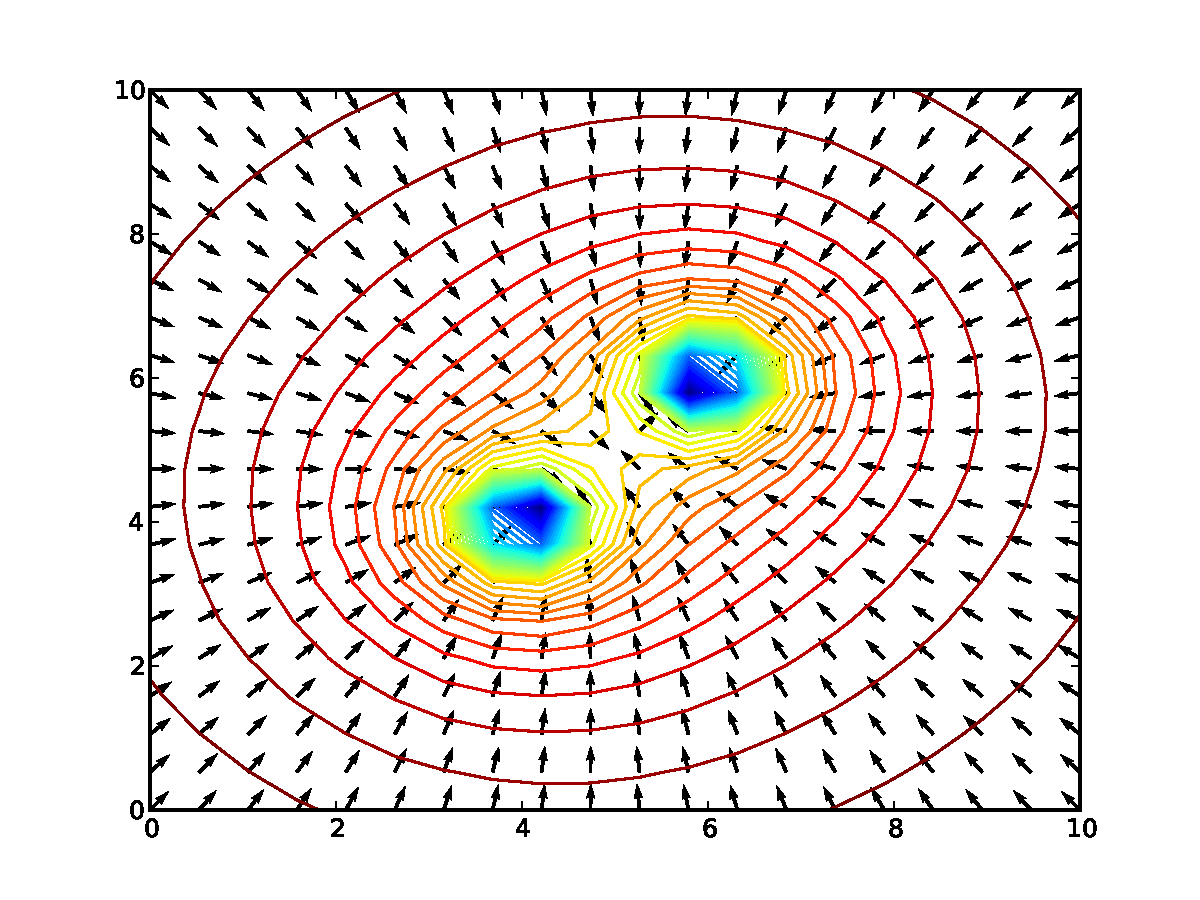
\includegraphics[width=0.65\textwidth]
	{./pictures/demo2_02.pdf}
	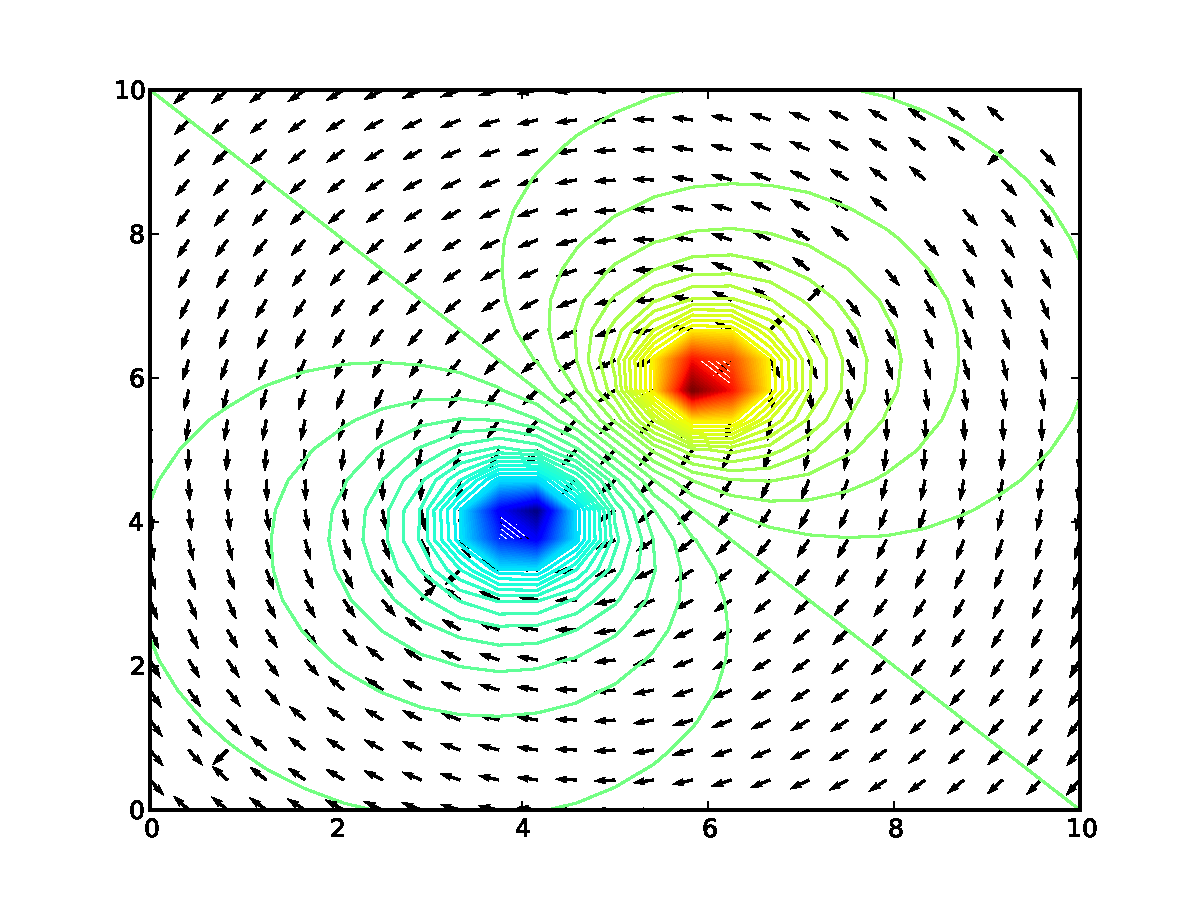
\includegraphics[width=0.65\textwidth]
	{./pictures/demo2_02(2).pdf}

	\caption{\small{Líneas de campo y equipotenciales de dos cargas 
	puntuales iguales. Con iguales signos (Superior) y con signos opuestos
	(Inferior).}}
	
	\label{fig:field_lines}
\end{figure}
%.........................................................................

A continuación se detalla cada parte del anterior script


%ccccccccccccccccccccccccccccccccccccccccccccccccccccccccccccccccccccccccc
%DEMO 2_01
\begin{listing}[style=python, numbers = none]
#Potencial de una particula puntual cargada
def Phi( r, rp, q ):
    phi = 1/(4*np.pi*eps0)*q/np.linalg.norm( r - rp )
    return phi

#Campo electrico de una particula puntual cargada
def Electric( r, rp, q ):
    E = 1/(4*np.pi*eps0)*q*(r - rp)/np.linalg.norm( r - rp )**3
    return E
\end{listing}
%ccccccccccccccccccccccccccccccccccccccccccccccccccccccccccccccccccccccccc
En estas líneas se definen la forma funcional del potencial y el campo
eléctrico asociados a una partícula puntual. Los argumentos \texttt{r} y
\texttt{rp} corresponden a los vectores donde se evalúan los campos y al 
vector posición de la partícula, respectivamente. Como tercer argumento se
da la carga eléctrica \texttt{q}. En el computo del campo eléctrico se usa
la función \texttt{norm} del paquete \texttt{linalg} de la librería \numpy
para calcular la norma del vector $\bds r - \bds r_p$.


%ccccccccccccccccccccccccccccccccccccccccccccccccccccccccccccccccccccccccc
%DEMO 2_01
\begin{listing}[style=python, numbers = none]
#Permitividad del vacio
eps0 = 8.85418e-12
#Resolucion de graficas
Nres = 25
#Coordenada X
Xarray = np.linspace( 0, 10, Nres )
#Coordenada Y
Yarray = np.linspace( 0, 10, Nres )
#Construccion de la cuadricula
X, Y = plt.meshgrid( Xarray, Yarray )
\end{listing}
%ccccccccccccccccccccccccccccccccccccccccccccccccccccccccccccccccccccccccc
Se define la permitividad del vacío en unidades SI y la resolución
espacial de la malla donde serán evaluadas funciones. Finalmente usando
la función \texttt{linspace} de la librería \numpy se construyen los 
arreglos asociados a cada eje espacial, de \texttt{0} a \texttt{10} metros
con una resolución de \texttt{Nres} divisiones, y luego usando la función
\texttt{meshgrid} de la librería \matplotlib se construyen las matrices de 
coordenadas, necesarias para la graficación de los campos.


%ccccccccccccccccccccccccccccccccccccccccccccccccccccccccccccccccccccccccc
%DEMO 2_01
\begin{listing}[style=python, numbers = none]
#CONSTRUCCION DE CAMPO E Y POTENCIAL PHI, PARTICULA 1
#Carga electrica
q1 = -1
#Posicion particula
rp1 = np.array( [4,4] )
#Incializacion Potencial Electrico
phi1 = np.zeros( (Nres,Nres) )
#Incializacion Campo Electrico
E1x = np.ones( (Nres,Nres) )
E1y = np.ones( (Nres,Nres) )
#Calculo Potencial Electrico y Campo Electrico
for i in xrange(Nres):
    for j in xrange(Nres):
	r = np.array( [Xarray[i], Yarray[j]] )
	phi1[i,j] = Phi( r, rp1, q1 )
	E = Electric( r, rp1, q1 )
	E1x[i,j], E1y[i,j] = E/np.linalg.norm(E)
\end{listing}
%ccccccccccccccccccccccccccccccccccccccccccccccccccccccccccccccccccccccccc
En esta parte se define y construye todas las propiedades físicas de la 
partícula 1. Inicialmente se define la carga \texttt{q1} y su posición
\texttt{rp1}. Posteriormente se inicializan las matrices donde se van a 
mapear los valores de los campos, primero el potencial como \texttt{phi1 = 
np.zeros( (Nres,Nres) )}, para esto se usa la función \texttt{zeros} de 
\numpy y se da como argumentos la dimensión $N_{res}\times N_{res}$ de la
matriz. De igual forma, usando la función \texttt{ones} de \numpy se 
inicializan las matrices asociadas a la componente $x$ y $y$ del campo 
$\bds E$. 

\

Usando los ciclos \textbf{\texttt{for}} de \python se hace un barrido de 
todas las matrices, tanto de las columnas como de las filas. Cada posición 
\texttt{i,j} está asociada a una coordenada $\bds r_{ij} = x_i\bds i + 
y_j\bds j$, en el código \texttt{r = np.array( [Xarray[i], Yarray[j]] )}.
Finalmente se calcula el potencial en este punto del espacio $\bds r_{ij}$
como \texttt{phi1[i,j] = Phi( r, rp1, q1 )} y cada componente del campo 
eléctrico \texttt{E1x[i,j]} y \texttt{E1y[i,j]}. Es importante mencionar
que lo único importante para definir las líneas de campo eléctrico es la
dirección local de $\bds E(\bds r_{ij})$, por esta razón se realiza la
normalización \texttt{E/np.linalg.norm(E)}, almacenando así el vector 
unitario que indica la dirección local del campo. Esto se repite para la
carga 2.


%ccccccccccccccccccccccccccccccccccccccccccccccccccccccccccccccccccccccccc
%DEMO 2_01
\begin{listing}[style=python, numbers = none]
#CONSTRUCCION DE CAMPO E Y POTENCIAL PHI, TOTAL
phi_tot = phi1 + phi2
#Incializacion Campo Electrico
Ex_tot = np.ones( (Nres,Nres) )
Ey_tot = np.ones( (Nres,Nres) )
#Calculo Potencial Electrico y Campo Electrico Total
for i in xrange(Nres):
    for j in xrange(Nres):
	E = np.array( [E1x[i,j] + E2x[i,j], \
	E1y[i,j] + E2y[i,j]] )
	E = E/np.linalg.norm(E)
	Ex_tot[i,j], Ey_tot[i,j] = E 
\end{listing}
%ccccccccccccccccccccccccccccccccccccccccccccccccccccccccccccccccccccccccc
Una vez calculados los campos asociados a ambas partículas, se procede a 
calcular los campos totales de toda la distribución. Para esto se tiene
en cuenta el principio de superposición, obteniendo el potencial total como
\texttt{phi\_tot = phi1 + phi2}. En el caso del campo eléctrico total 
$\bds E_{tot}$ se debe usar de nuevo dos ciclos \textbf{\texttt{for}} para
calcular la nueva normalización del campo 

\[ \bds E_{tot}(\bds r_{ij}) = \frac{\bds E_1(\bds r_{ij}) + \bds E_2(\bds r_{ij})}
{|\bds E_1(\bds r_{ij})+\bds E_2(\bds r_{ij})|} \]

Obteniendo así la dirección local en $\bds r_{ij}$ del campo total.


%ccccccccccccccccccccccccccccccccccccccccccccccccccccccccccccccccccccccccc
%DEMO 2_01
\begin{listing}[style=python, numbers = none]
#Grafica de equipotenciales
plt.contour(X, Y, phi_tot, 100)
#Grafica de lineas de campo
plt.quiver( X, Y, Ey_tot, Ex_tot)
\end{listing}
%ccccccccccccccccccccccccccccccccccccccccccccccccccccccccccccccccccccccccc
Finalmente se usan las funciones \texttt{contour} y \texttt{quiver} de la
librería \matplotlib para graficar los campos totales. La función 
\texttt{contour} tiene como argumentos las matrices de coordenadas \texttt{X} 
y \texttt{Y}, la matriz del campo total \texttt{phi\_tot} y el número de 
equipotenciales a graficar. Para la función \texttt{quiver} los argumentos
son las matrices de coordenadas \texttt{X} y \texttt{Y} nuevamente y las 
matrices de las componentes $x$ y $y$ del campo eléctrico total $\bds E_{tot}$.


 
\rule{14cm}{0.5mm}
%*************************************************************************




\
%*************************************************************************
\section{Demostración 3: Billar Electrostático}
\label{sec:DEMO2_03}
\rule{14cm}{0.5mm}

En cada demostración serán introducidos gradualmente conceptos más avanzados 
de programación. Para este caso será usado un integrador numérico para 
solucionar el problema electrostático de 3 cuerpos y será representado en 
una animación 3D la evolución del sistema usando la librería \mayavi.

\

El problema de tres cuerpos es un problema clásico en física y para el cual
no existe solución numérica salvo casos muy particulares. Es por esta 
razón que el uso de métodos numéricos es completamente necesario. 

\

Para simplificar el sistema y sin pérdida de generalidad, se asumirá una 
interacción en dos dimensiones y una geometría rectangular. Por este 
motivo se ha denominado billar electrostático, ya que este satisface la 
descripción del sistema (ver figura \ref{fig:biliard}).


%.........................................................................
%Electrostatic biliard
\begin{figure}[htbp]
	\centering
	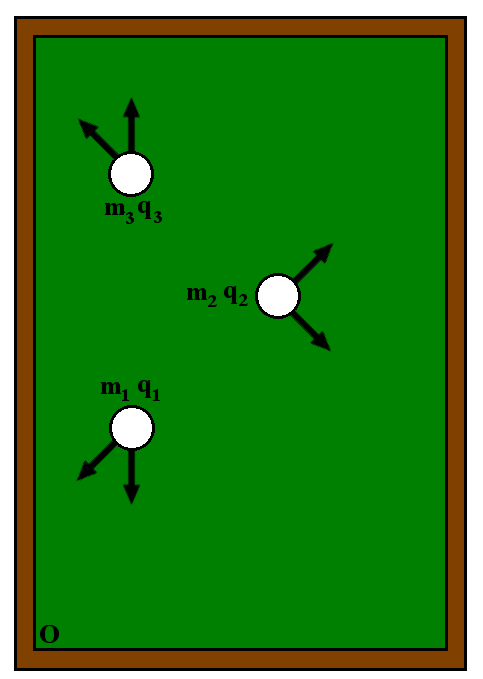
\includegraphics[width=0.4\textwidth]
	{./pictures/billiards.png}

	\caption{\small{Billar electrostático con 3 bolas cargadas interactuando
	en dos dimensiones.}}
	
	\label{fig:biliard}
\end{figure}
%.........................................................................


La ecuación de movimiento para la bola $i$ está dada por 


%.........................................................................
%Fields of point particles distribution
\eq{eq:Movement_ball}
{ m_i\dtot{^2 \bds r_i}{t^2} = \sum_{j,j\neq i}^3 \frac{1}{4\pi \epsilon_0} 
\frac{q_i q_j}{|\bds r_i - \bds r_j|^3}(\bds r_i - \bds r_j) }
%.........................................................................
donde se considera la interacción con las otras dos bolas y además se asume
una distribución de carga uniforme, de tal forma que el campo eléctrico 
generado pueda ser reemplazado por el de una carga equivalente puntual.

\

Introduciendo la velocidad de la bola $i$ como $\bds v_i = d\bds r_i/dt$,
las ecuaciones de movimiento para todo el sistema pueden escribirse en
coordenadas cartesianas como

%.........................................................................
%Equation system of biliard
\begin{eqnarray}
\label{eq:balls_eqs_i}
\dtot{x_1}{t} &=& v_{x,1}										 \\
\dtot{y_1}{t} &=& v_{y,1} 										 \\
\dtot{v_{x,1}}{t} &=& \frac{q_1}{4\pi \epsilon_0 m} 
\cor{ \frac{q_2}{|\bds r_1 - \bds r_2|^3}\pr{x_1 - x_2} + 
\frac{q_3}{|\bds r_1 - \bds r_3|^3}\pr{x_1 - x_3} }				 \\
\dtot{v_{y,1}}{t} &=& \frac{q_1}{4\pi \epsilon_0 m}
\cor{ \frac{q_2}{|\bds r_1 - \bds r_2|^3}\pr{y_1 - y_2} + 
\frac{q_3}{|\bds r_1 - \bds r_3|^3}\pr{y_1 - y_3} }				 \\
\dtot{x_2}{t} &=& v_{x,2}										 \\
\dtot{y_2}{t} &=& v_{y,2} 										 \\
\dtot{v_{x,2}}{t} &=& \frac{q_2}{4\pi \epsilon_0 m} 
\cor{ \frac{q_1}{|\bds r_2 - \bds r_1|^3}\pr{x_2 - x_1} + 
\frac{q_3}{|\bds r_2 - \bds r_3|^3}\pr{x_2 - x_3} }				 \\
\dtot{v_{y,2}}{t} &=& \frac{q_2}{4\pi \epsilon_0 m}
\cor{ \frac{q_1}{|\bds r_2 - \bds r_1|^3}\pr{y_2 - y_1} + 
\frac{q_3}{|\bds r_2 - \bds r_3|^3}\pr{y_2 - y_3} }				 \\
\dtot{x_3}{t} &=& v_{x,3}										 \\
\dtot{y_3}{t} &=& v_{y,3} 										 \\
\dtot{v_{x,3}}{t} &=& \frac{q_3}{4\pi \epsilon_0 m} 
\cor{ \frac{q_1}{|\bds r_3 - \bds r_1|^3}\pr{x_3 - x_1} + 
\frac{q_2}{|\bds r_3 - \bds r_2|^3}\pr{x_3 - x_2} }				 \\
\label{eq:balls_eqs_f}
\dtot{v_{y,3}}{t} &=& \frac{q_3}{4\pi \epsilon_0 m}
\cor{ \frac{q_1}{|\bds r_3 - \bds r_1|^3}\pr{y_3 - y_1} + 
\frac{q_2}{|\bds r_3 - \bds r_2|^3}\pr{y_3 - y_2} }
\end{eqnarray}
%.........................................................................


El siguiente script de \python realiza la integración numérica del sistema
y grafica las trayectorias de cada bola.


%ccccccccccccccccccccccccccccccccccccccccccccccccccccccccccccccccccccccccc
%DEMO 2_03_1
\begin{listing}[style=python]
#!/usr/bin/env python
#==========================================================
# DEMOSTRACION 3: Parte 1
# Solucion numerica de problema de 3 cuerpos 
# electrostaticos
#==========================================================
from __future__ import division
import numpy as np
import matplotlib.pylab as plt
import scipy.integrate as integ
from RungeKutta4 import rk4_step

#Ecuaciones de movimiento
def dF(Y, t):
    #Posicion X particula 1
    x1 = Y[0]
    #Posicion Y particula 1
    y1 = Y[1]
    #Velocidad X particula 1
    vx1 = Y[2]
    #Velocidad Y particula 1
    vy1 = Y[3]
    
    #Posicion X particula 2
    x2 = Y[4]
    #Posicion Y particula 2
    y2 = Y[5]
    #Velocidad X particula 2
    vx2 = Y[6]
    #Velocidad Y particula 2
    vy2 = Y[7]
    
    #Posicion X particula 3
    x3 = Y[8]
    #Posicion Y particula 3
    y3 = Y[9]
    #Velocidad X particula 3
    vx3 = Y[10]
    #Velocidad Y particula 3
    vy3 = Y[11]
    
    #Modulo distancia entre particula 1 y 2
    r12 = np.linalg.norm( [x1-x2, y1-y2] )
    #Modulo distancia entre particula 1 y 3
    r13 = np.linalg.norm( [x1-x3, y1-y3] )
    #Modulo distancia entre particula 2 y 3
    r23 = np.linalg.norm( [x2-x3, y2-y3] )
    
    #Derivada dx/dt particula 1
    dx1 = vx1
    #Derivada dy/dt particula 1
    dy1 = vy1
    #Derivada d vx/dt particula 1
    dvx1 = q1/(4*np.pi*eps0*m1)*( q2/r12**3*(x1-x2) + \
    q3/r13**3*(x1-x3) )
    #Derivada d vy/dt particula 1
    dvy1 = q1/(4*np.pi*eps0*m1)*( q2/r12**3*(y1-y2) + \
    q3/r13**3*(y1-y3) )
    
    #Derivada dx/dt particula 2
    dx2 = vx2
    #Derivada dy/dt particula 2
    dy2 = vy2
    #Derivada d vx/dt particula 2
    dvx2 = q2/(4*np.pi*eps0*m2)*( q1/r12**3*(x2-x1) + \
    q3/r23**3*(x2-x3) )
    #Derivada d vy/dt particula 2
    dvy2 = q2/(4*np.pi*eps0*m2)*( q1/r12**3*(y2-y1) + \
    q3/r23**3*(y2-y3) )
    
    #Derivada dx/dt particula 3
    dx3 = vx3
    #Derivada dy/dt particula 3
    dy3 = vy3
    #Derivada d vx/dt particula 3
    dvx3 = q3/(4*np.pi*eps0*m3)*( q1/r13**3*(x3-x1) + \
    q2/r23**3*(x3-x2) )
    #Derivada d vy/dt particula 3
    dvy3 = q3/(4*np.pi*eps0*m3)*( q1/r13**3*(y3-y1) + \
    q2/r23**3*(y3-y2) )

    #Derivadas
    return np.array([ dx1, dy1, dvx1, dvy1, \
    dx2, dy2, dvx2, dvy2, \
    dx3, dy3, dvx3, dvy3 ])
    

#CONSTANTES
#Permitividad del vacio
eps0 = 8.85418e-12
#Ancho de la mesa
ancho = 1.2
#Largo de la mesa
largo = 2.4

#CONDICIONES BOLA 1
#masa
m1 = 0.1
#carga
q1 = 5e-5
#radio 
r1 = 0.05
#posicion inicial
x10 = 0.1
y10 = 0.1
#velocidad inicial
vx10 = 5.0
vy10 = 5.0

#CONDICIONES BOLA 2
#masa
m2 = 0.1
#carga
q2 = 5e-5
#radio 
r2 = 0.05
#posicion inicial
x20 = 0.3
y20 = 0.1
#velocidad inicial
vx20 = -5.0
vy20 = 5.0

#CONDICIONES BOLA 3
#masa
m3 = 0.1
#carga
q3 = 5e-5
#radio 
r3 = 0.05
#posicion inicial
x30 = 0.2
y30 = 0.2
#velocidad inicial
vx30 = -1.0
vy30 = 5.0

#INTEGRACION DEL SISTEMA
#tiempo maximo a integrar
t_max = 10
#salto del tiempo
t_step = 0.001
#condiciones iniciales
cond_ini = [ x10, y10, vx10, vy10, \
x20, y20, vx20, vy20, \
x30, y30, vx30, vy30]
#tiempo de evaluacion
tiempo = np.arange( 0, t_max, t_step )
#integracion del sistema
solucion = []
Y = cond_ini
for t in tiempo:
    Y = rk4_step( dF, Y, t, t_step )
    #Condiciones de colision con la mesa
    if Y[0] < r1 or Y[0] >= ancho-r1:
	Y[2] = -Y[2]
    if Y[4] < r2 or Y[4] >= ancho-r2:
	Y[6] = -Y[6]
    if Y[8] < r3 or Y[8] >= ancho-r3:
	Y[10] = -Y[10]
	
    if Y[1] < r1 or Y[1] >= largo-r1:
	Y[3] = -Y[3]
    if Y[5] < r2 or Y[5] >= largo-r2:
	Y[7] = -Y[7]
    if Y[9] < r3 or Y[9] >= largo-r3:
	Y[11] = -Y[11]

    solucion.append( Y )

#resultado de integracion
x1_t, y1_t, vx1_t, vy1_t, \
x2_t, y2_t, vx2_t, vy2_t, \
x3_t, y3_t, vx3_t, vy3_t = \
np.transpose( solucion )

#Guardando archivo de datos
np.savetxt( 'trayectorias.txt', np.transpose([tiempo,\
x1_t, y1_t, x2_t, y2_t, x3_t, y3_t]) )

#Grafica de trayectorias
plt.plot( x1_t, y1_t, label='particula 1' )
plt.plot( x2_t, y2_t, label='particula 2')
plt.plot( x3_t, y3_t, label='particula 3')

#Formato de grafica
plt.xlim( (0,ancho) )
plt.ylim( (0,largo) )
plt.grid()
plt.legend()
plt.show()
\end{listing}
%ccccccccccccccccccccccccccccccccccccccccccccccccccccccccccccccccccccccccc

\newpage
Se obtiene la siguiente figura con las trayectorias de cada bola


%.........................................................................
%Electrostatic biliard trayectories
\begin{figure}[htbp]
	\centering
	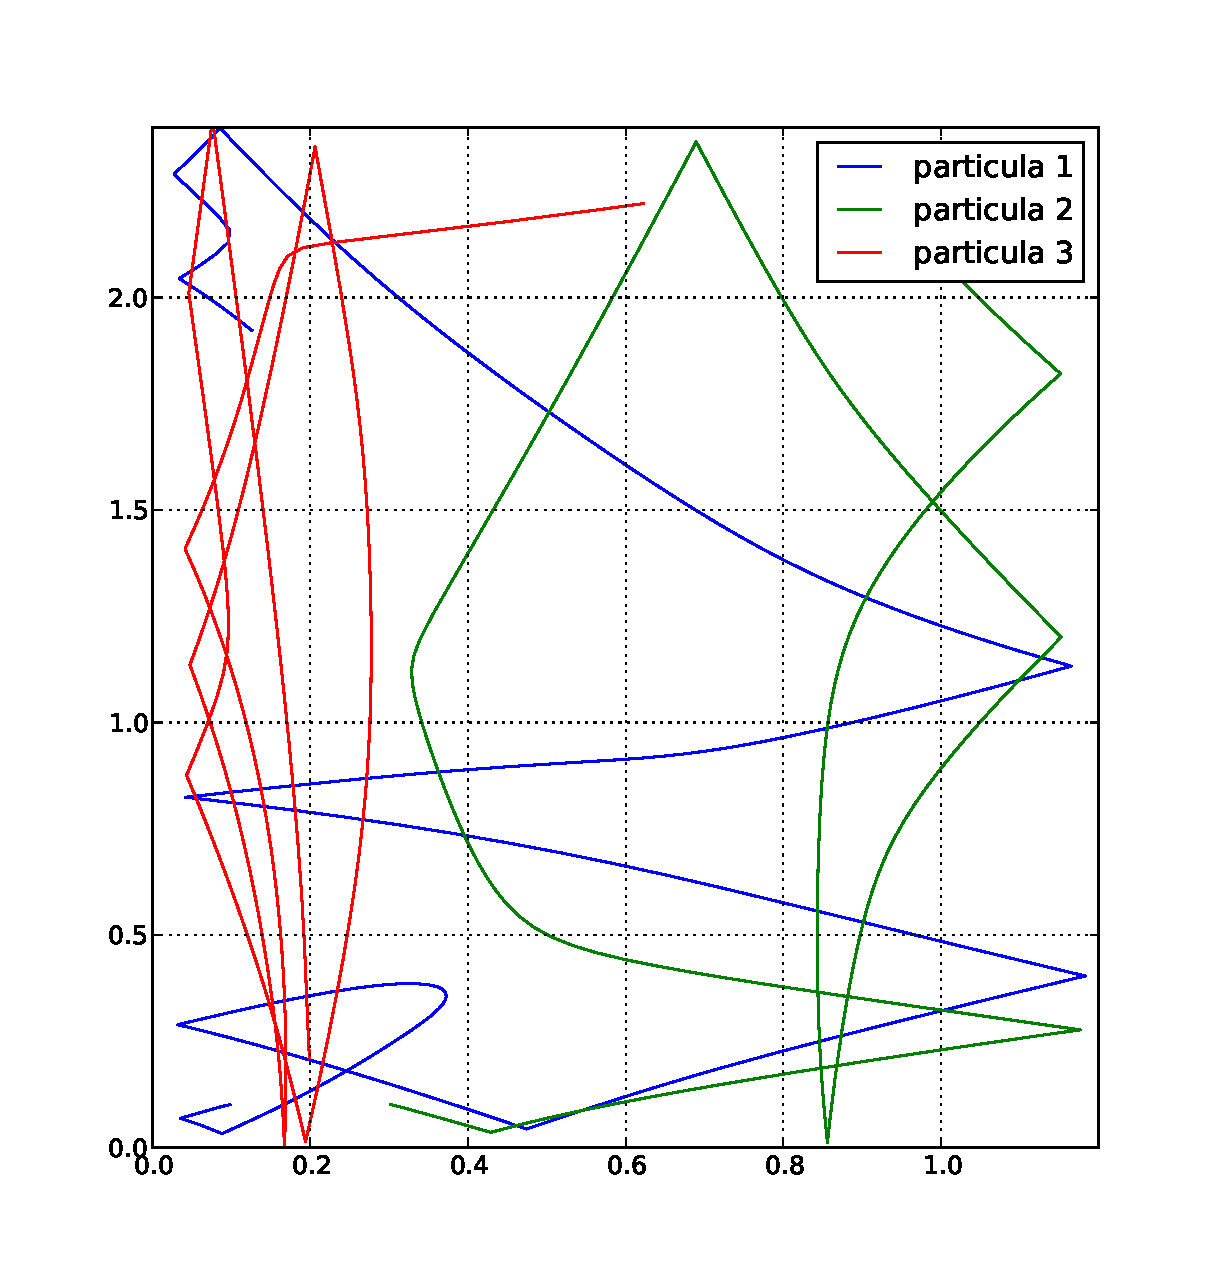
\includegraphics[width=0.75\textwidth]
	{./pictures/demo2_03(1).pdf}

	\caption{\small{Trayectoria calculada numéricamente de las tres bolas
	del problema.}}
	
	\label{fig:balls_trayectories}
\end{figure}
%.........................................................................


y un archivo de texto \texttt{trayectorias.txt} con las soluciones del 
sistema en el formato \texttt{[tiempo, x1, y1, x2, y2, x3, y3]}, donde 
\texttt{xi, yi} denontan la posición $x$ y $y$ de la bola i. 

\

A continuación se explica cada parte del código


%ccccccccccccccccccccccccccccccccccccccccccccccccccccccccccccccccccccccccc
%DEMO 2_03_1
\begin{listing}[style=python, numbers = none]
from __future__ import division
import numpy as np
import matplotlib.pylab as plt
from RungeKutta4 import rk4_step
\end{listing}
%ccccccccccccccccccccccccccccccccccccccccccccccccccccccccccccccccccccccccc
En estas líneas iniciales se cargan las librerías estándares ya conocidas.
En la última línea \texttt{from RungeKutta4 import rk4\_step} se importa
la función \texttt{rk4\_step} que corresponde al integrador numérico para 
solucionar las ecuaciones de movimiento. Este se puede encontrar en el 
archivo \texttt{RungeKutta4.py}. Note que a pesar de no ser una librería, 
\python permite tratarlo como tal, e importar funciones específicas desde
un archivo externo.


%ccccccccccccccccccccccccccccccccccccccccccccccccccccccccccccccccccccccccc
%DEMO 2_03_1
\begin{listing}[style=python, numbers = none]
#Ecuaciones de movimiento
def dF(Y, t):
    #Posicion X particula 1
    x1 = Y[0]
    #Posicion Y particula 1
    y1 = Y[1]
    #Velocidad X particula 1
    vx1 = Y[2]
    #Velocidad Y particula 1
    vy1 = Y[3]
    
    #Posicion X particula 2
    x2 = Y[4]
    #Posicion Y particula 2
    y2 = Y[5]
    #Velocidad X particula 2
    vx2 = Y[6]
    #Velocidad Y particula 2
    vy2 = Y[7]
    
    #Posicion X particula 3
    x3 = Y[8]
    #Posicion Y particula 3
    y3 = Y[9]
    #Velocidad X particula 3
    vx3 = Y[10]
    #Velocidad Y particula 3
    vy3 = Y[11]
    
    #Modulo distancia entre particula 1 y 2
    r12 = np.linalg.norm( [x1-x2, y1-y2] )
    #Modulo distancia entre particula 1 y 3
    r13 = np.linalg.norm( [x1-x3, y1-y3] )
    #Modulo distancia entre particula 2 y 3
    r23 = np.linalg.norm( [x2-x3, y2-y3] )
    
    #Derivada dx/dt particula 1
    dx1 = vx1
    #Derivada dy/dt particula 1
    dy1 = vy1
    #Derivada d vx/dt particula 1
    dvx1 = q1/(4*np.pi*eps0*m1)*( q2/r12**3*(x1-x2) + \
    q3/r13**3*(x1-x3) )
    #Derivada d vy/dt particula 1
    dvy1 = q1/(4*np.pi*eps0*m1)*( q2/r12**3*(y1-y2) + \
    q3/r13**3*(y1-y3) )
    
    #Derivada dx/dt particula 2
    dx2 = vx2
    #Derivada dy/dt particula 2
    dy2 = vy2
    #Derivada d vx/dt particula 2
    dvx2 = q2/(4*np.pi*eps0*m2)*( q1/r12**3*(x2-x1) + \
    q3/r23**3*(x2-x3) )
    #Derivada d vy/dt particula 2
    dvy2 = q2/(4*np.pi*eps0*m2)*( q1/r12**3*(y2-y1) + \
    q3/r23**3*(y2-y3) )
    
    #Derivada dx/dt particula 3
    dx3 = vx3
    #Derivada dy/dt particula 3
    dy3 = vy3
    #Derivada d vx/dt particula 3
    dvx3 = q3/(4*np.pi*eps0*m3)*( q1/r13**3*(x3-x1) + \
    q2/r23**3*(x3-x2) )
    #Derivada d vy/dt particula 3
    dvy3 = q3/(4*np.pi*eps0*m3)*( q1/r13**3*(y3-y1) + \
    q2/r23**3*(y3-y2) )

    #Derivadas
    return np.array([ dx1, dy1, dvx1, dvy1, \
    dx2, dy2, dvx2, dvy2, \
    dx3, dy3, dvx3, dvy3 ])
\end{listing}
%ccccccccccccccccccccccccccccccccccccccccccccccccccccccccccccccccccccccccc
En esta parte se define la función dinámica del sistema, la cual contiene
todas las derivadas asociadas a las ecuaciones de movimiento 
\ref{eq:balls_eqs_i} - \ref{eq:balls_eqs_f}. El arreglo \texttt{Y} contiene 
todas las variables del sistema en el orden $x_i, y_i, v_{xi}, v_{yi}$ para 
cada bola. En las primeras líneas se extrae entonces cada valor para las 
bolas, por ejemplo para la bola 1 se tiene \texttt{x1 = Y[0]}, 
\texttt{y1 = Y[1]}, \texttt{vx1 = Y[2]} y \texttt{vy1 = Y[3]} y de igual 
forma para las otras dos.

\

Luego se calcula el módulo de distancia entre los vectores de posición de
cada bola, por ejemplo entre las bolas 1 y 2 se tiene
\texttt{r12 = np.linalg.norm( [x1-x2, y1-y2] )}, de igual forma para las 
bolas 1 y 3 y las bolas 2 y 3..

\

Finalmente se calculan las derivadas de las variables de cada bola acorde
a las ecuaciones de movimiento y se retorna un arreglo con todas estas en 
el mismo orden en que están en el arreglo inicial \texttt{Y}. \texttt{
np.array([ dx1, dy1, dvx1, dvy1, dx2, dy2, dvx2, dvy2, dx3, dy3, dvx3, dvy3 ])}.
La función \texttt{array} de la librería \numpy se usa con el fin de 
convertir una lista en un objeto matemático tipo vector.


%ccccccccccccccccccccccccccccccccccccccccccccccccccccccccccccccccccccccccc
%DEMO 2_03_1
\begin{listing}[style=python, numbers = none]
#CONSTANTES
#Permitividad del vacio
eps0 = 8.85418e-12
#Ancho de la mesa
ancho = 1.2
#Largo de la mesa
largo = 2.4
\end{listing}
%ccccccccccccccccccccccccccccccccccccccccccccccccccccccccccccccccccccccccc
Se definen las constantes del sistema, la permitividad del vacío $\epsilon_0$,
y las dimensiones de la mesa, todo en unidades SI.


%ccccccccccccccccccccccccccccccccccccccccccccccccccccccccccccccccccccccccc
%DEMO 2_03_1
\begin{listing}[style=python, numbers = none]
#CONDICIONES BOLA 1
#masa
m1 = 0.1
#carga
q1 = 5e-5
#radio 
r1 = 0.05
#posicion inicial
x10 = 0.1
y10 = 0.1
#velocidad inicial
vx10 = 5.0
vy10 = 5.0
\end{listing}
%ccccccccccccccccccccccccccccccccccccccccccccccccccccccccccccccccccccccccc
Las condiciones físicas de la bola 1 son definidas en estas líneas. Se dan
valores a la masa, la carga, el radio de la bola, su posición inicial y su 
velocidad inicial, todo en unidades SI. Esto se repite para las otras dos
bolas.


%ccccccccccccccccccccccccccccccccccccccccccccccccccccccccccccccccccccccccc
%DEMO 2_03_1
\begin{listing}[style=python, numbers = none]
#INTEGRACION DEL SISTEMA
#tiempo maximo a integrar
t_max = 10
#salto del tiempo
t_step = 0.001
#condiciones iniciales
cond_ini = [ x10, y10, vx10, vy10, \
x20, y20, vx20, vy20, \
x30, y30, vx30, vy30]
#tiempo de evaluacion
tiempo = np.arange( 0, t_max, t_step )
\end{listing}
%ccccccccccccccccccccccccccccccccccccccccccccccccccccccccccccccccccccccccc
Se procede con la integración de la ecuaciones del sistema. Primero se 
define el tiempo máximo en el cual se desea evolucionar las bolas, en este
caso $10$ s. Luego se define el paso de integración, que corresponde al 
valor del intervalo de tiempo en que se van almacenando los valores $x$ y 
$y$ de las bolas. Se construye un arreglo con las condiciones iniciales de 
posición y velocidad definidas para cada bola \texttt{cond\_ini}. Finalmente
se construye el arreglo con todos los tiempos en los que se desea calcular 
las soluciones \texttt{tiempo = np.arange( 0, t\_max, t\_step )}


%ccccccccccccccccccccccccccccccccccccccccccccccccccccccccccccccccccccccccc
%DEMO 2_03_1
\begin{listing}[style=python, numbers = none]
#integracion del sistema
solucion = []
Y = cond_ini
for t in tiempo:
    Y = rk4_step( dF, Y, t, t_step )
    #Condiciones de colision con la mesa
    if Y[0] < r1 or Y[0] >= ancho-r1:
	Y[2] = -Y[2]
    if Y[4] < r2 or Y[4] >= ancho-r2:
	Y[6] = -Y[6]
    if Y[8] < r3 or Y[8] >= ancho-r3:
	Y[10] = -Y[10]
	
    if Y[1] < r1 or Y[1] >= largo-r1:
	Y[3] = -Y[3]
    if Y[5] < r2 or Y[5] >= largo-r2:
	Y[7] = -Y[7]
    if Y[9] < r3 or Y[9] >= largo-r3:
	Y[11] = -Y[11]

    solucion.append( Y )

#resultado de integracion
x1_t, y1_t, vx1_t, vy1_t, \
x2_t, y2_t, vx2_t, vy2_t, \
x3_t, y3_t, vx3_t, vy3_t = \
np.transpose( solucion )
\end{listing}
%ccccccccccccccccccccccccccccccccccccccccccccccccccccccccccccccccccccccccc
Se crea un arreglo vacío \texttt{solucion = []} sonde se almacenan las 
soluciones de la trayectorias en cada tiempo. Luego se define el arreglo 
\texttt{Y} con las condiciones iniciales \texttt{Y = cond\_ini} para 
posteriormente comenzar una iteración en el tiempo, calculando en cada ciclo
las nuevas soluciones. Se usa entonces la función \texttt{rk4\_step} del 
archivo \texttt{RungeKutta4.py} para calcular la solución del siguiente 
tiempo \texttt{t+t\_step}, \texttt{Y = rk4\_step( dF, Y, t, t\_step )}. 
Los argumentos de esta función son entonces, el nombre de la función con 
las ecuaciones de movimiento \texttt{dF}, las soluciones en el tiempo 
anterior \texttt{Y}, el tiempo actual \texttt{t} y el salto de tiempo de 
integración \texttt{t\_step}. Luego en se extrae del arreglo (matriz) 
\texttt{solucion} cada una de las soluciones en el tiempo, para esto se
usa la función \texttt{transpose} de \numpy en orden para tomar los datos 
acorde a las columnas y no a las filas.



%ccccccccccccccccccccccccccccccccccccccccccccccccccccccccccccccccccccccccc
%DEMO 2_03_1
\begin{listing}[style=python, numbers = none]
#Guardando archivo de datos
np.savetxt( 'trayectorias.txt', np.transpose([tiempo,\
x1_t, y1_t, x2_t, y2_t, x3_t, y3_t]) )

#Grafica de trayectorias
plt.plot( x1_t, y1_t, label='particula 1' )
plt.plot( x2_t, y2_t, label='particula 2')
plt.plot( x3_t, y3_t, label='particula 3')

#Formato de grafica
plt.xlim( (0,ancho) )
plt.ylim( (0,largo) )
plt.grid()
plt.legend()
plt.show()
\end{listing}
%ccccccccccccccccccccccccccccccccccccccccccccccccccccccccccccccccccccccccc
En esta última parte se guarda en un archivo externo \texttt{trayectorias.txt}
las trayectorias calculadas en el formato \texttt{tiempo, x1\_t, y1\_t, 
x2\_t, y2\_t, x3\_t, y3\_t}. Para esto se usa la función \texttt{savetxt}
de la librería \numpy, esta tiene como argumentos el nombre del archivo 
externo a guardar. y los datos calculados. Estos se dan en un arreglo 
(matriz) que se transpone de nuevo para obtener los datos acorde a las 
columnas y no a las filas. En lo siguiente se grafica la trayectoria 
de cada bola usando la función \texttt{plot} de \matplotlib. Finalmente
se da formato a la ventana de graficación y se muestra en pantalla.

\

\

En la segunda parte de esta demostración se usa el archivo de texto guardado
en el primer script para representar en una animación 3D el sistema físico.
Para esto se usa la librería \mayavi y el script es el siguiente.



%ccccccccccccccccccccccccccccccccccccccccccccccccccccccccccccccccccccccccc
%DEMO 2_03_2
\begin{listing}[style=python]
#!/usr/bin/env python
#==========================================================
# DEMOSTRACION 3: Parte 2
# Solucion numerica de problema de 3 cuerpos 
# electrostaticos. Animacion 3D
#==========================================================
import numpy as np
import enthought.tvtk.tools.visual as visual

#Cargando datos de las bolas
tiempo, x1_t, y1_t, x2_t, y2_t, x3_t, y3_t = \
np.transpose( np.loadtxt('trayectorias.txt') )

#CONSTANTES
#Ancho de la mesa
ancho = 1.2
#Largo de la mesa
largo = 2.4
#Grosor de los muros del billar
grosor = 0.1
#Radio bola 1
r1 = 0.05
#Radio bola 2
r2 = 0.05
#Radio bola 3
r3 = 0.05

#Creando bola 1
bola1 = visual.sphere( radius=r1, color=(1.0, 1.0, 1.0) )
bola1.pos = [ 0., 0., 0. ]
bola1.t = 0
bola1.dt = 1

#Creando bola 2
bola2 = visual.sphere( radius=r2, color=(1.0, 1.0, 1.0) )
bola2.pos = [ 0., 0., 0. ]
bola2.t = 0
bola2.dt = 1

#Creando bola 1
bola3 = visual.sphere( radius=r3, color=(1.0, 1.0, 1.0) )
bola3.pos = [ 0., 0., 0. ]
bola3.t = 0
bola3.dt = 1

#Creando mesa
mesa = visual.box( pos=(ancho/2., largo/2., -grosor/2.), \
size=(ancho, largo, grosor), color=(0.0, 0.3, 0.0) )

muro_l = visual.box( pos=(-grosor/2., largo/2., 0.0), \
size=(grosor, largo + 2*grosor, grosor), \
color=(0.6, 0.3, 0.0) )
muro_r = visual.box( pos=(ancho+grosor/2., largo/2., 0.0), \
size=(grosor, largo + 2*grosor, grosor), \
color=(0.6, 0.3, 0.0) )
muro_d = visual.box( pos=(ancho/2., -grosor/2., 0.0), \
size=(ancho + 2*grosor, grosor, grosor), \
color=(0.6, 0.3, 0.0) )
muro_u = visual.box( pos=(ancho/2., largo+grosor/2., 0.0), \
size=(ancho + 2*grosor, grosor, grosor), \
color=(0.6, 0.3, 0.0) )


#ITERACION DEL SISTEMA
def anim(): 
    #Evolucion de la bola 1
    bola1.t = bola1.t + bola1.dt
    i = bola1.t
    bola1.pos = visual.vector( x1_t[i], y1_t[i], r1 )
    
    #Evolucion de la bola 2
    bola2.t = bola2.t + bola2.dt
    i = bola2.t
    bola2.pos = visual.vector( x2_t[i], y2_t[i], r2 )
    
    #Evolucion de la bola 3
    bola3.t = bola3.t + bola3.dt
    i = bola3.t
    bola3.pos = visual.vector( x3_t[i], y3_t[i], r3 )
    
a = visual.iterate(10, anim)
visual.show()
\end{listing}
%ccccccccccccccccccccccccccccccccccccccccccccccccccccccccccccccccccccccccc

El resultado obtenido está ilustrado en la siguiente figura


%.........................................................................
%Electrostatic biliard trayectories
\begin{figure}[htbp]
	\centering
	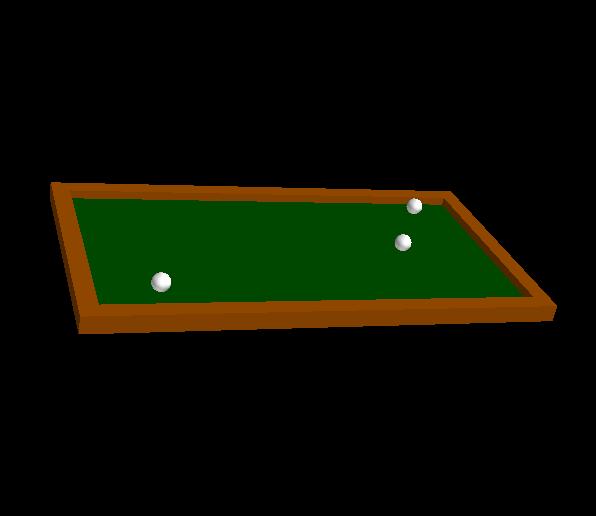
\includegraphics[width=0.75\textwidth]
	{./pictures/billiards_animated.png}

	\caption{\small{Animación 3D del sistema de billar electrostático 
	usando \mayavi.}}
	
	\label{fig:balls_trayectories_3D}
\end{figure}
%.........................................................................


A continuación se describe el código anterior


%ccccccccccccccccccccccccccccccccccccccccccccccccccccccccccccccccccccccccc
%DEMO 2_03_2
\begin{listing}[style=python, numbers = none]
import numpy as np
import enthought.tvtk.tools.visual as visual
\end{listing}
%ccccccccccccccccccccccccccccccccccccccccccccccccccccccccccccccccccccccccc
En estas primeras líneas se carga las diferentes librerías necesarias para
esta segunda parte de la demostración. Primero la librería \numpy ya 
conocida y luego se carga el paquete \texttt{visual} de la librería \mayavi.
\textbf{Nota:} para algunas versiones de \mayavi la forma correcta de 
cargar esta librería es \texttt{import tvtk.tools.visual as visual}.


%ccccccccccccccccccccccccccccccccccccccccccccccccccccccccccccccccccccccccc
%DEMO 2_03_2
\begin{listing}[style=python, numbers = none]
#Cargando datos de las bolas
tiempo, x1_t, y1_t, x2_t, y2_t, x3_t, y3_t = \
np.transpose( np.loadtxt('trayectorias.txt') )
\end{listing}
%ccccccccccccccccccccccccccccccccccccccccccccccccccccccccccccccccccccccccc
Usando la función \texttt{loadtxt} de la librería \numpy se cargan los 
datos guardados en el primer script. Como único argumento se tiene el 
nombre del archivo. De nuevo se usa la función \texttt{transpose} para 
cargar los datos acorde a las columnas y no a las filas.


%ccccccccccccccccccccccccccccccccccccccccccccccccccccccccccccccccccccccccc
%DEMO 2_03_2
\begin{listing}[style=python, numbers = none]

#CONSTANTES
#Ancho de la mesa
ancho = 1.2
#Largo de la mesa
largo = 2.4
#Grosor de los muros del billar
grosor = 0.1
#Radio bola 1
r1 = 0.05
#Radio bola 2
r2 = 0.05
#Radio bola 3
r3 = 0.05
\end{listing}
%ccccccccccccccccccccccccccccccccccccccccccccccccccccccccccccccccccccccccc
En esta parte se definen nuevamente los parámetros físicos del sistema
asociados longitudes.


%ccccccccccccccccccccccccccccccccccccccccccccccccccccccccccccccccccccccccc
%DEMO 2_03_2
\begin{listing}[style=python, numbers = none]
#Creando bola 1
bola1 = visual.sphere( radius=r1, color=(1.0, 1.0, 1.0) )
bola1.pos = [ 0., 0., 0. ]
bola1.t = 0
bola1.dt = 1
\end{listing}
%ccccccccccccccccccccccccccccccccccccccccccccccccccccccccccccccccccccccccc
Usando la función \texttt{sphere} del módulo \texttt{visual} de \mayavi se
construye la bola 1 del sistema. Como argumentos de la función 
\texttt{sphere} se da su radio \texttt{radius} y el color como \texttt{color}. 
El formato de color está en código RGB donde un color es un arreglo de 
tres números que toman valores entre 0 y 1. La primera componente determina 
la cantidad de rojo, con 0 nulo y 1 máximo, de igual forma la segunda 
componente para el verde y la tercera para el azul. Como ejemplos, el 
rojo equivale a \texttt{(1,0,0)}, mientras que el negro \texttt{(0,0,0)}, 
el blanco \texttt{(1,1,1)}, el violeta \texttt{(1,0,1)}, etc. Luego se da 
una posición inicial de la bola, la cual no es definitiva y es cambiada 
cuando se cargue la trayectoria correspondiente. Finalmente se da el tiempo 
inicial y el salto de tiempo \texttt{dt}. Este salto de tiempo no 
corresponde al salto de tiempo físico del script anterior, en vez de esto, 
este debe ser un entero ($1$) debido a que corresponde a la posición 
en los arreglos de las trayectorias entre tiempo y tiempo. Esto se repite
para las otras 2 bolas.


%ccccccccccccccccccccccccccccccccccccccccccccccccccccccccccccccccccccccccc
%DEMO 2_03_2
\begin{listing}[style=python, numbers = none]
#Creando mesa
mesa = visual.box( pos=(ancho/2., largo/2., -grosor/2.), \
size=(ancho, largo, grosor), color=(0.0, 0.3, 0.0) )
\end{listing}
%ccccccccccccccccccccccccccccccccccccccccccccccccccccccccccccccccccccccccc
En estas líneas se define el objeto asociado a la mesa de billar. Para esto
se usa la función \texttt{box} de \texttt{visual} de la siguiente forma 
\texttt{mesa = visual.box( pos= (ancho /2., largo/2., -grosor/2.), 
size=(ancho, largo,}\\ \texttt{grosor), color=(0.0, 0.3, 0.0) )}. Como primer argumento 
se da la posición del centro geométrico de la caja, el segundo argumento 
es un arreglo con el grosor, el alto y el ancho de la caja, en el mismo 
orden. Finalmente se da el color en formato RGB, con \texttt{(0.0, 0.3, 0.0)} 
equivalente al color verde oscuro. De igual forma se crean los límites de 
la mesa.


%ccccccccccccccccccccccccccccccccccccccccccccccccccccccccccccccccccccccccc
%DEMO 2_03_2
\begin{listing}[style=python, numbers = none]
#ITERACION DEL SISTEMA
def anim(): 
    #Evolucion de la bola 1
    bola1.t = bola1.t + bola1.dt
    i = bola1.t
    bola1.pos = visual.vector( x1_t[i], y1_t[i], r1 )
\end{listing}
%ccccccccccccccccccccccccccccccccccccccccccccccccccccccccccccccccccccccccc
Se define la función \texttt{anim} encargada de trazar la trayectoria de 
cada bola. Inicialmente se aumenta el tiempo asociado a la bola al 
siguiente valor \texttt{t+dt}. Luego se define el índice \texttt{i} en los
arreglos de datos asociado a los datos del tiempo actual. Finalmente se 
actualiza la posición de la bola 1 con el atributo \texttt{pos} del objeto
\texttt{bola1} de tal forma que \texttt{bola1.pos = visual.vector( 
x1\_t[i], y1\_t[i], r1 )}. Se debe tener en cuenta que la posición en el 
eje \texttt{z} debe ser el radio de la bola \texttt{r1} y no \texttt{0},
esto para que la bola no intercepte la mesa sino que esté sobre ella.


%ccccccccccccccccccccccccccccccccccccccccccccccccccccccccccccccccccccccccc
%DEMO 2_03_2
\begin{listing}[style=python, numbers = none]
a = visual.iterate(10, anim)
visual.show()
\end{listing}
%ccccccccccccccccccccccccccccccccccccccccccccccccccccccccccccccccccccccccc
Finalmente se ejecuta la función \texttt{visual.iterate}, esta presenta
la animación del sistema de forma gráfica. Como primer argumento se da el 
tiempo en milisegundos que se quiere entre cada iteración del sistema, así
por ejemplo un valor bajo como \texttt{10} implica un tiempo de $10$ ms 
entre frame y frame, produciendo una animación más fluida, mientras que un
valor más alto como \texttt{50} produce una animación en cámara lenta. El 
segundo argumento es el nombre de la función donde está la evolución de los
péndulos, en este caso \texttt{anim}.


\rule{14cm}{0.5mm}
%*************************************************************************